\begin{figure}[ht]
\centering
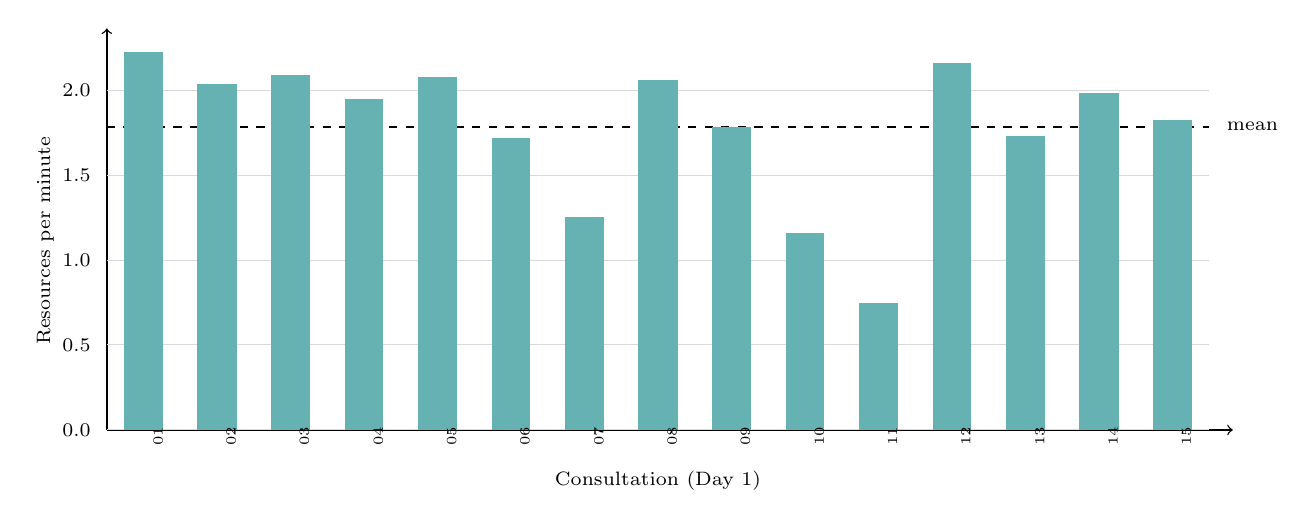
\begin{tikzpicture}[x=1cm,y=1cm]
\draw[->, line width=0.5pt] (1.00,0.80) -- (1.00,5.90);
\draw[->, line width=0.5pt] (1.00,0.80) -- (15.30,0.80);
\draw[gray!30] (1.00,0.80) -- (15.00,0.80);
\node[anchor=east,font=\scriptsize] at (0.92,0.80) {0.0};
\draw[gray!30] (1.00,1.88) -- (15.00,1.88);
\node[anchor=east,font=\scriptsize] at (0.92,1.88) {0.5};
\draw[gray!30] (1.00,2.95) -- (15.00,2.95);
\node[anchor=east,font=\scriptsize] at (0.92,2.95) {1.0};
\draw[gray!30] (1.00,4.03) -- (15.00,4.03);
\node[anchor=east,font=\scriptsize] at (0.92,4.03) {1.5};
\draw[gray!30] (1.00,5.11) -- (15.00,5.11);
\node[anchor=east,font=\scriptsize] at (0.92,5.11) {2.0};
\draw[dashed, line width=0.6pt] (1.00,4.65) -- (15.00,4.65);
\node[anchor=west,font=\scriptsize] at (15.10,4.65) {mean};
\fill[teal!60] (1.22,0.80) rectangle (1.71,5.60);
\node[anchor=north,font=\tiny,rotate=90] at (1.47,0.72) {01};
\fill[teal!60] (2.15,0.80) rectangle (2.65,5.19);
\node[anchor=north,font=\tiny,rotate=90] at (2.40,0.72) {02};
\fill[teal!60] (3.09,0.80) rectangle (3.58,5.31);
\node[anchor=north,font=\tiny,rotate=90] at (3.33,0.72) {03};
\fill[teal!60] (4.02,0.80) rectangle (4.51,5.00);
\node[anchor=north,font=\tiny,rotate=90] at (4.27,0.72) {04};
\fill[teal!60] (4.95,0.80) rectangle (5.45,5.28);
\node[anchor=north,font=\tiny,rotate=90] at (5.20,0.72) {05};
\fill[teal!60] (5.89,0.80) rectangle (6.38,4.51);
\node[anchor=north,font=\tiny,rotate=90] at (6.13,0.72) {06};
\fill[teal!60] (6.82,0.80) rectangle (7.31,3.51);
\node[anchor=north,font=\tiny,rotate=90] at (7.07,0.72) {07};
\fill[teal!60] (7.75,0.80) rectangle (8.25,5.24);
\node[anchor=north,font=\tiny,rotate=90] at (8.00,0.72) {08};
\fill[teal!60] (8.69,0.80) rectangle (9.18,4.65);
\node[anchor=north,font=\tiny,rotate=90] at (8.93,0.72) {09};
\fill[teal!60] (9.62,0.80) rectangle (10.11,3.30);
\node[anchor=north,font=\tiny,rotate=90] at (9.87,0.72) {10};
\fill[teal!60] (10.55,0.80) rectangle (11.05,2.41);
\node[anchor=north,font=\tiny,rotate=90] at (10.80,0.72) {11};
\fill[teal!60] (11.49,0.80) rectangle (11.98,5.46);
\node[anchor=north,font=\tiny,rotate=90] at (11.73,0.72) {12};
\fill[teal!60] (12.42,0.80) rectangle (12.91,4.53);
\node[anchor=north,font=\tiny,rotate=90] at (12.67,0.72) {13};
\fill[teal!60] (13.35,0.80) rectangle (13.85,5.08);
\node[anchor=north,font=\tiny,rotate=90] at (13.60,0.72) {14};
\fill[teal!60] (14.29,0.80) rectangle (14.78,4.74);
\node[anchor=north,font=\tiny,rotate=90] at (14.53,0.72) {15};
\node[rotate=90,font=\scriptsize] at (0.22,3.20) {Resources per minute};
\node[font=\scriptsize] at (8.00,0.15) {Consultation (Day 1)};
\end{tikzpicture}
\caption{Clinical-resource density for Step~5 outputs, normalized by consultation duration. Variation here reflects output volume relative to recording length, not verified semantic completeness.}
\label{fig:extraction-resource-density}
\end{figure}
